\documentclass{article}
\usepackage{fontenc}
\usepackage{graphicx}
\usepackage[a4paper,margin=1in]{geometry}
\usepackage{amsmath,amssymb}
\usepackage{enumitem}
\usepackage{fancyhdr}
\usepackage{circuitikz}
\usepackage{titlesec}
\date{\today}
\geometry{top=1in, bottom=1in, left=1in, right=1in}
\pagestyle{empty}
\begin{document}
\thispagestyle{fancy}
\fancyhf{}
\fancyhead[L]{
\includegraphics[width=8cm, height=1.7cm]{IIITB-COMET-Logo.png}}
\fancyhead[R]{

   Name:Namathoti Srinivas\\
   Batch:COMETFWC036\\
   Date:09 August 2025\\
}
\renewcommand{\headrulewidth}{0.4pt}
\fancyfoot[c]{\thepage}
\vspace{1cm}
\begin{center}
$$\textbf{\Huge GATE EE 2010 PAPER}$$
\end{center}
The following karnaugh map represents a function \(F\)
\begin{figure}[h!]
    \centering
    % First image
    
\includegraphics[width=0.6\textwidth]{Kmap.jpg}
\end{figure}
\textbf{52.} A minimized form of the function \( F \) is
\begin{enumerate}[label=(\Alph*)]
    \item \( F = XY + YZ \)
    \item \( F = X Y + Y Z \)
    \item \( F = X Y + Y Z \)
    \item \( F = X Y Z \)
\end{enumerate}
\textbf{Solution:}
The minterms where $F=1$ are:
$$
m_0 = \overline{X} \, \overline{Y} \, \overline{Z}, \quad
m_1 = \overline{X} \, \overline{Y} \, Z, \quad
m_3 = \overline{X} \, Y \, Z, \quad
m_7 = X \, Y \, Z
$$
Simplifying, we get:
$$
F = \overline{X} \, \overline{Y} + YZ
$$

\textbf{53.} Which of the following circuits is a realization of the above function \(F\)

\begin{figure}[h!]
    \centering
    % Second image
    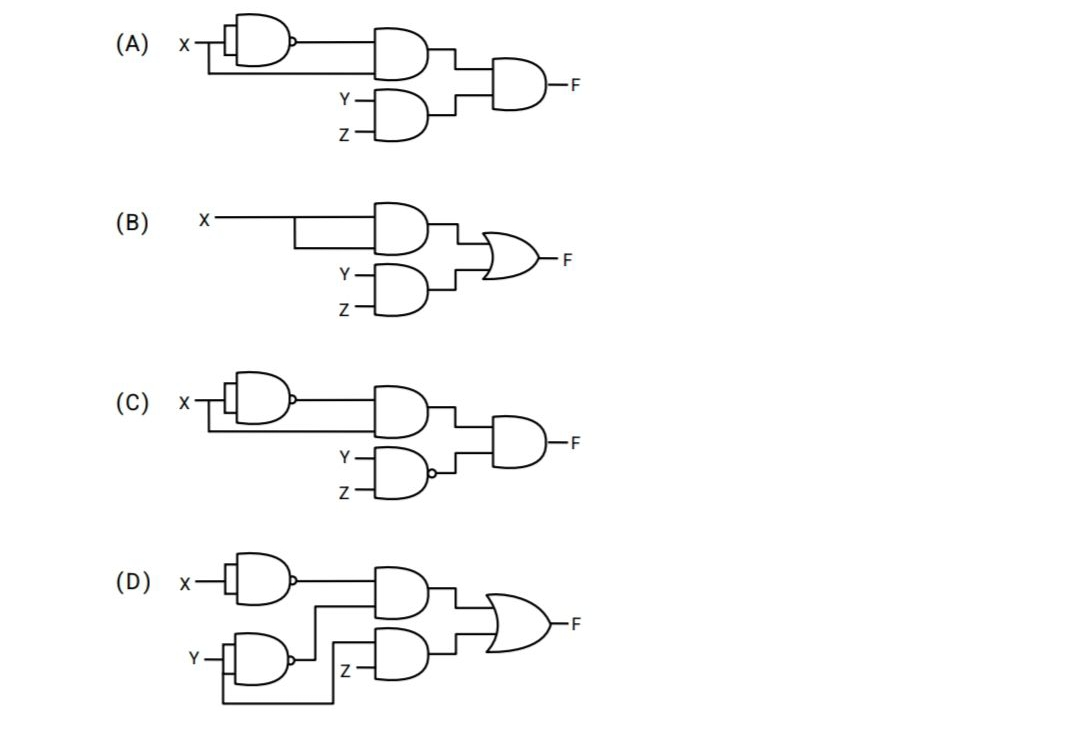
\includegraphics[width=0.8\textwidth]{DigitalCircuits.jpg}
\end{figure}
\newpage\textbf{Solution:}
  We know that the function \(F=\overline{X} \, \overline{Y}+YZ\)\\ 
  Based on the function\(F\) the realized circuit is  
\begin{figure}[h!]
    \centering
    % Third image
    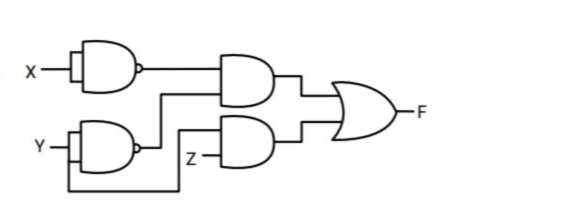
\includegraphics[width=0.8\textwidth]{RealizedCircuit.jpg}
\end{figure}
\end{document}
